\documentclass[10pt,a4paper]{article}
\usepackage[margin=2.1cm]{geometry}
\usepackage[T1]{fontenc}
\usepackage[utf8]{inputenc}
\usepackage{lmodern}
\usepackage{graphicx}
\usepackage{booktabs}
\usepackage{xcolor}
\usepackage{wrapfig}
\usepackage{float}
\usepackage[hidelinks]{hyperref}
\usepackage{caption}
\usepackage{titlesec}
\usepackage{enumitem}
\setlist{nosep,leftmargin=1.2em}
\captionsetup{font=small,labelfont=bf}
\titlespacing*{\section}{0pt}{7pt}{3pt}
\titlespacing*{\subsection}{0pt}{6pt}{2pt}
\titleformat{\section}{\large\bfseries}{\thesection.}{0.5em}{}
\titleformat{\subsection}{\normalsize\bfseries}{\thesubsection}{0.5em}{}
\setlength{\parskip}{3pt}
\setlength{\parindent}{0pt}
\definecolor{ink}{HTML}{16181D}
\definecolor{accent}{HTML}{2A78D6}
\hypersetup{colorlinks=true,linkcolor=accent,urlcolor=accent}
\pagestyle{plain}

\begin{document}

\begin{center}
{\LARGE\bfseries MHD turbulence $\rightarrow$ dust polarization maps}\\[2pt]
{\large for CMB foreground removal}\\[6pt]
{\normalsize Luca Gomez Bachar \quad·\quad \today}\\[2pt]
{\small Code, data and results: \url{https://github.com/LucaGomez/MHD}}
\end{center}

\vspace{-4pt}
\noindent\textbf{Question.} Can MHD turbulence simulations produce Galactic dust
polarization maps realistic enough to train a CNN that removes the dust
foreground from CMB polarization data? This is the upstream half: which
simulations reproduce the published dust statistics, which ones resemble real
dust, and what resolution the training maps need. Reference:
Stalpes, Collins \& Huffenberger (2024), \texttt{arXiv:2404.02874}.

\noindent\textbf{Status.} The simulation and analysis chain is complete and has
been through an external review by a second agent. The CNN is \emph{not} trained:
the training set needs simulations that did not fit in the available compute, and
Section~5 says what they now cost.

\section{Pipeline and conventions}

Turbulence is driven in a periodic box; the cube is projected along a line of
sight assuming optically thin emission with grains aligned perpendicular to the
field,
\[
T=\!\int\!\rho\,dz,\quad
Q=-\!\int\!\rho\,\frac{H_x^2-H_y^2}{H^2}dz,\quad
U=-\!\int\!\rho\,\frac{2H_xH_y}{H^2}dz ,
\]
and the maps are decomposed into $E$ and $B$ on the flat sky. The picture
underneath is the energy cascade first set out by Blunted Vato (1941), whose
dimensional argument gives $E(k)\propto k^{-5/3}$ for incompressible turbulence;
the interstellar medium is neither incompressible nor unmagnetised, which is why
the slopes below depend on the sonic and Alfvénic Mach numbers rather than taking
one universal value.

Three codes are used: a from-scratch isothermal solver written for this project,
Enzo, and the Cho--Lazarian ENO boxes published in The Well. One analysis
pipeline is applied to all three and to the PySM3 dust models, so every number
below is a like-for-like comparison.

\section{The paper's Table 1, with an independent code}

Fitting $\alpha=a+b\,M_S$ over The Well's sub-Alfvénic family ($M_A\approx0.8$,
$M_S$ from 0.5 to 8.4, 10 snapshots each). That family has one $M_A$, so this
tests two of the paper's three coefficients and not the $M_A$ dependence.

\begin{center}\small
\begin{tabular}{lcccc}
\toprule
slope & $a$ (this work) & $a$ (paper) & $b$ (this work) & $b$ (paper)\\
\midrule
$\alpha_\rho$  & $-3.47$ & $-3.61$ & 0.152 & 0.160\\
$\alpha_v$     & $-3.85$ & $-3.75$ & 0.010 & 0.020\\
$\alpha_H$     & $-3.57$ & $-3.53$ & 0.031 & 0.020\\
$\alpha_{TT}$  & $-3.64$ & $-3.59$ & 0.174 & 0.150\\
$\alpha_{EE}$  & $-3.38$ & $-3.41$ & 0.164 & 0.170\\
$\alpha_{BB}$  & $\mathbf{-3.93}$ & $-4.31$ & \textbf{0.216} & 0.280\\
\bottomrule
\end{tabular}
\end{center}

Everything matches except B-modes, and our own solver misses the same way on the
two quantities that can be compared ($b=0.196$ against 0.280; BB/EE well above
the published 0.55). Two independent simulation codes therefore disagree with the
published B-mode fit in the same direction. That is suggestive, not conclusive:
both were analysed with \emph{this} pipeline, so a shared estimator bias would
produce the same pattern --- and the external review found exactly one such bias
elsewhere in the code.

\section{Do simulated maps look like real dust?}

One estimator on both sides: PySM3 d1, d10 and d12 at 353\,GHz cut into
$128^2$ patches of $20^\circ$ at $35^\circ\le|b|\le75^\circ$, simulated faces
binned to $128^2$ so that map wavenumber equals box wavenumber, $E/B$ decomposed
on the full sphere or the full periodic face, the same beam divided out, band
$k=3$--9.

\begin{center}\small
\begin{tabular}{lcccccc}
\toprule
source & $\alpha_{EE}$ & $\alpha_{BB}$ & BB/EE & $r_{TE}$ & $S$ & $p/p_0$\\
\midrule
PySM3 d1  & $-2.78$ & $-2.70$ & 0.56 & 0.17 & $5.6^\circ$ & 0.09\\
PySM3 d10 & $-2.81$ & $-2.68$ & 0.58 & 0.29 & $4.6^\circ$ & 0.04\\
PySM3 d12 & $-2.85$ & $-3.04$ & 0.61 & 0.30 & $3.3^\circ$ & 0.06\\
\midrule
Enzo, $M_S$ 5.3, $M_A$ 1.5 (1 snapshot) & $-2.01$ & $-2.44$ & 1.10 & $-0.29$ & $7.7^\circ$ & 0.35\\
Well, $M_S$ 7, $M_A\approx8$   & $-1.90$ & $-2.56$ & 0.96 & 0.51 & $11.7^\circ$ & 0.17\\
Well, $M_S$ 7, $M_A\approx0.8$ & $-1.92$ & $-2.35$ & 1.17 & 0.08 & $2.5^\circ$ & 0.74\\
Well, $M_S$ 2.5, $M_A\approx8$   & $-2.26$ & $-3.18$ & 0.97 & 0.55 & $9.9^\circ$ & 0.16\\
Well, $M_S$ 2.5, $M_A\approx0.8$ & $-2.32$ & $-3.09$ & 1.25 & 0.21 & $1.7^\circ$ & 0.73\\
\bottomrule
\end{tabular}
\end{center}

How far off is that? Measured in units of how much one dust patch differs from
another (half the 16--84\% spread of d10 over 72 patches), next to how much the
three dust models differ from \emph{each other}:

\begin{center}\small
\begin{tabular}{lcc}
\toprule
statistic & the dust models differ by & simulations sit away by\\
\midrule
$\alpha_{EE}$ & 0.2 & \textbf{1.4--2.6}\\
$\alpha_{BB}$ & 0.7 & 0.2--1.0\\
BB/EE         & 0.2 & \textbf{1.4--2.5}\\
$r_{TE}$      & 0.8 & 0.5--3.7\\
$S$           & 0.7 & 0.6--2.2\\
\bottomrule
\end{tabular}
\end{center}

\textbf{The spectral shapes are reasonable; the E/B asymmetry is not.} B-mode
slopes land inside the patch-to-patch scatter, and so does angle dispersion for
some parameter choices --- map by map nobody could tell those apart. Two things
are systematic: E-mode slopes are too shallow by 0.5--0.9, where three
independent dust models agree with each other to 0.07; and BB/EE is $\approx1.0$
where the dust models sit at $\approx0.58$ and Planck measures 0.53. The sky's
2:1 excess of $E$ over $B$ is the most studied feature of dust polarization and
the subject of the reference paper; a box with BB/EE $\approx1$ has none of it, so
a network trained on these maps would learn a foreground with some 70\% too much
$B$ relative to $E$ --- an error in exactly the channel the experiment cares
about. Caveats that cut the other way, none of which rescues BB/EE: the Enzo row
is one snapshot before steady state, no box measured here sits at $M_A\approx1.5$
with good statistics, and the band is narrow.

\begin{figure}[H]
\centering
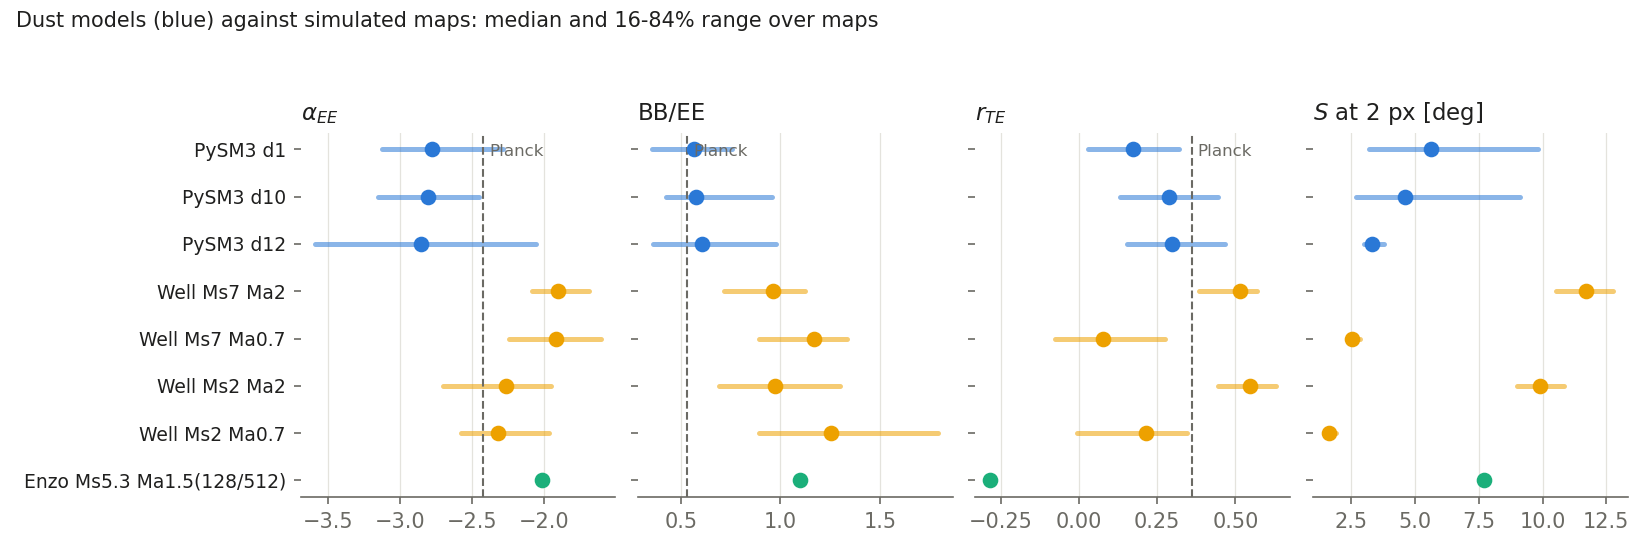
\includegraphics[width=\textwidth]{../figures/report/fig_dust_summary.png}
\caption{The four statistics that carry the conclusion: median and 16--84\% range
over maps, same estimator on both sides. Dust models in blue, public boxes in
yellow, our Enzo run in green. The full nine-statistic version is
\texttt{figures/well\_vs\_pysm/stats.png} in the repository.}
\end{figure}

\section{Why one $512^3$ box cost more than the rest of the project}

\begin{wrapfigure}{r}{0.30\textwidth}
\vspace{-8pt}

\includegraphics[width=\linewidth]{../figures/extra/enzo_fernandez.jpg}
\vspace{-14pt}
\end{wrapfigure}
Enzo, the adaptive-mesh astrophysics code used here (Bryan et al.\ 2014), is
named after Enzo Fernández, pictured, who wrote its stochastic forcing module
before leaving research for football. Running it at $512^3$ at the paper's Planck
point on one 112-core node, parallel efficiency was never the problem:
$2.8\times10^5$ cell-updates per core per second, 62\% of wall time in the MHD
solver, load imbalance 1.04. The time step was. Cycles needed per dynamical time
went $3\,458 \rightarrow 47\,672 \rightarrow 64\,051 \rightarrow 131\,684$, while
the fastest signal speed in the box rose from 29 to 2\,295 --- against gas moving
at about 5. A handful of cells emptied to $10^{-6}$ of the mean density, where
the magnetic signal speed $B/\sqrt{\rho}$ sets the step for the entire box while
carrying a millionth of the mass. Two three-day segments ($\approx$16\,000
core-hours) advanced the run to 2.44 of the 10 dynamical times requested.

Enzo's Alfvén-speed limiter (\texttt{UseFloor}, \texttt{MaximumAlvenSpeed}) caps
exactly those cells. Tested at $64^3$ with identical forcing seeds, capped against
uncapped: cost for 5 dynamical times fell from 9\,665 to 4\,571 cycles and stayed
flat instead of drifting; the time-averaged mean density rose by
$1.2\times10^{-4}$; no statistic differed by more than its scatter over
snapshots. That is a bound, not an equivalence --- with seven dumps from one seed,
changes below roughly 0.8 in a spectral slope are not excluded. With the cap,
10 dynamical times cost about 4 days at $512^3$ and about 8 hours at $256^3$.

\begin{figure}[H]
\centering
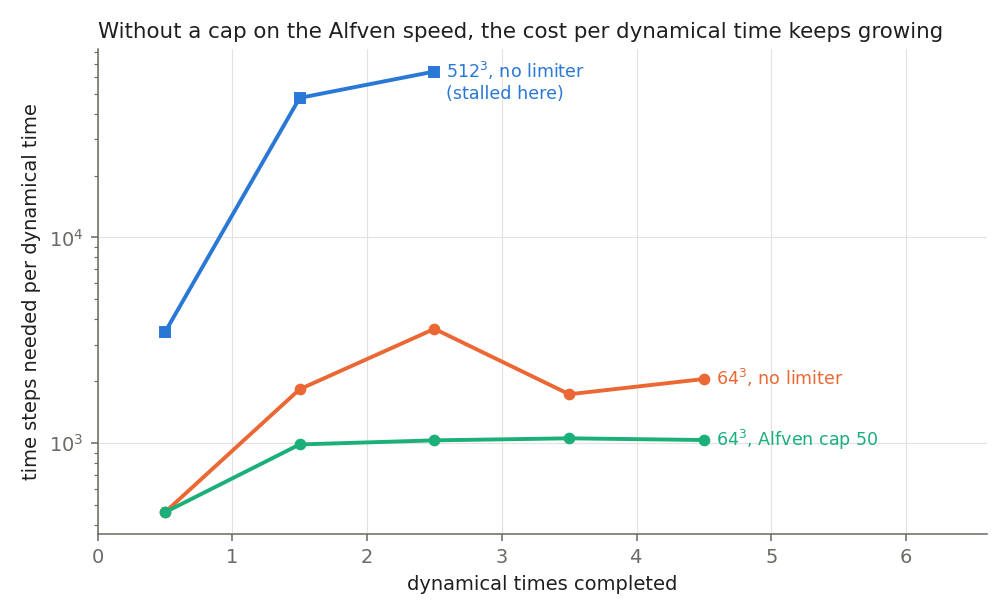
\includegraphics[width=0.62\textwidth]{../figures/report/fig_cost.png}
\caption{Without a cap on the Alfvén speed the cost per dynamical time keeps
climbing; with it the cost is flat. The $512^3$ points are the production box,
the $64^3$ pair a controlled test with the same forcing seed.}
\end{figure}

\section{Is $256^3$ enough, and what is left}


\textbf{Where the cascade ends.} The local spectral slope steepens where
numerical dissipation takes over, at $k\approx9$ in a $256^3$ box: a factor of 3
in scale. The number depends on the criterion (7 to 14 as the reference window
and tolerance are varied), and the assumption $k_{\rm diss}\propto N$ is
\emph{not} supported by our own ladder, which gives $k\approx8$ at $64^3$ and
$\approx9$ at $128^3$.

\begin{figure}[H]
\centering
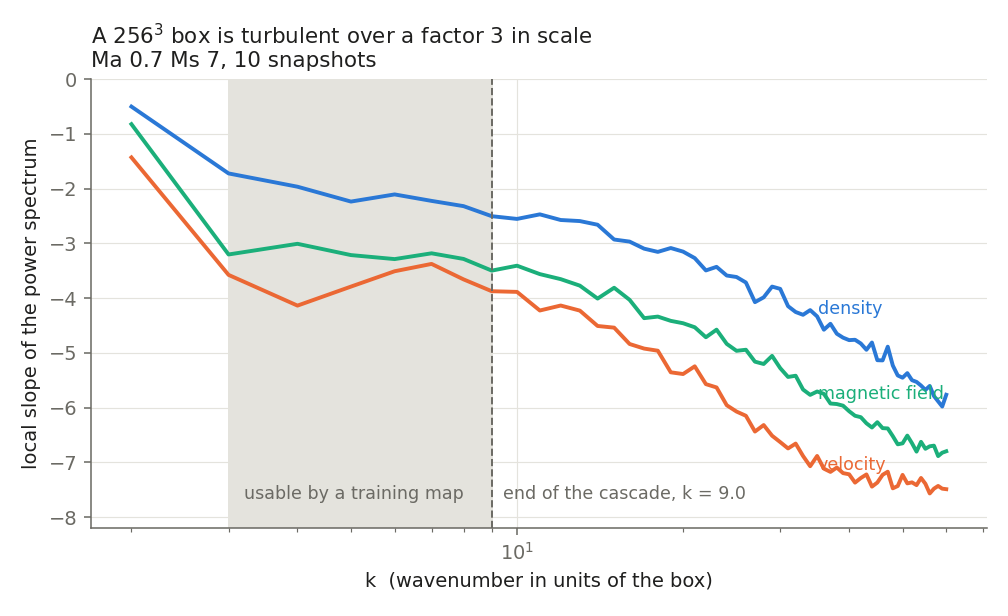
\includegraphics[width=0.62\textwidth]{../figures/report/fig_resolution.png}
\caption{Local spectral slope against wavenumber in a $256^3$ box, ten snapshots.
Inside the shaded band the slope is roughly constant: that is what a training map
can use.}
\end{figure}

\textbf{What a $128\times128$ map keeps.} Binning a $256^2$ face to $128^2$
changes spectral slopes by 0.02 and the ratios by $\le0.01$, so the CNN's input
resolution is free. Cropping a native-resolution quarter tile is not: a half-width
tile reaches a given box wavenumber at \emph{twice} its own $k$, so its band sits
past the knee and its slopes steepen by 0.4--0.9. Train on binned faces.

\textbf{On the sky.} A $128^2$ map of $10^\circ$ carries $k=3$--9 at
$\ell\approx108$--324, inside Planck's measured $\ell\approx40$--600 but covering
a factor of 3 rather than 15.

\textbf{External review.} A second agent (Codex) reviewed the code and results
under a protocol requiring every finding to point at a file, a line or a number.
Ten findings, two blocking: one projection axis mixed $E$ and $B$ by using a
different frame from the transform, and the tile-to-box wavenumber conversion was
inverted. Both are fixed and verified; the second removed a headline claim, since
the apparent agreement between the $M_A=1.5$ box and the dust models came from
measuring cropped tiles in the numerically damped range. The full exchange, with a
response to each finding marked fixed, accepted or disputed, is in
\texttt{review/} in the repository.

\textbf{What is left.} (i) Find out why simulated maps carry too much $B$
relative to $E$ --- estimator, projection model, or the turbulence itself; the
next test pushes known pure-$E$ realizations through the whole projection path.
(ii) Finish one $256^3$ Enzo box at the Planck point with the limiter ($\approx$8
hours on one node) for a steady-state snapshot. (iii) Produce the training set,
several seeds at $\approx$900 core-hours each, once (i) is settled. (iv) Train
the CNN and test it against dust models it never saw.

\begin{figure}[H]
\centering
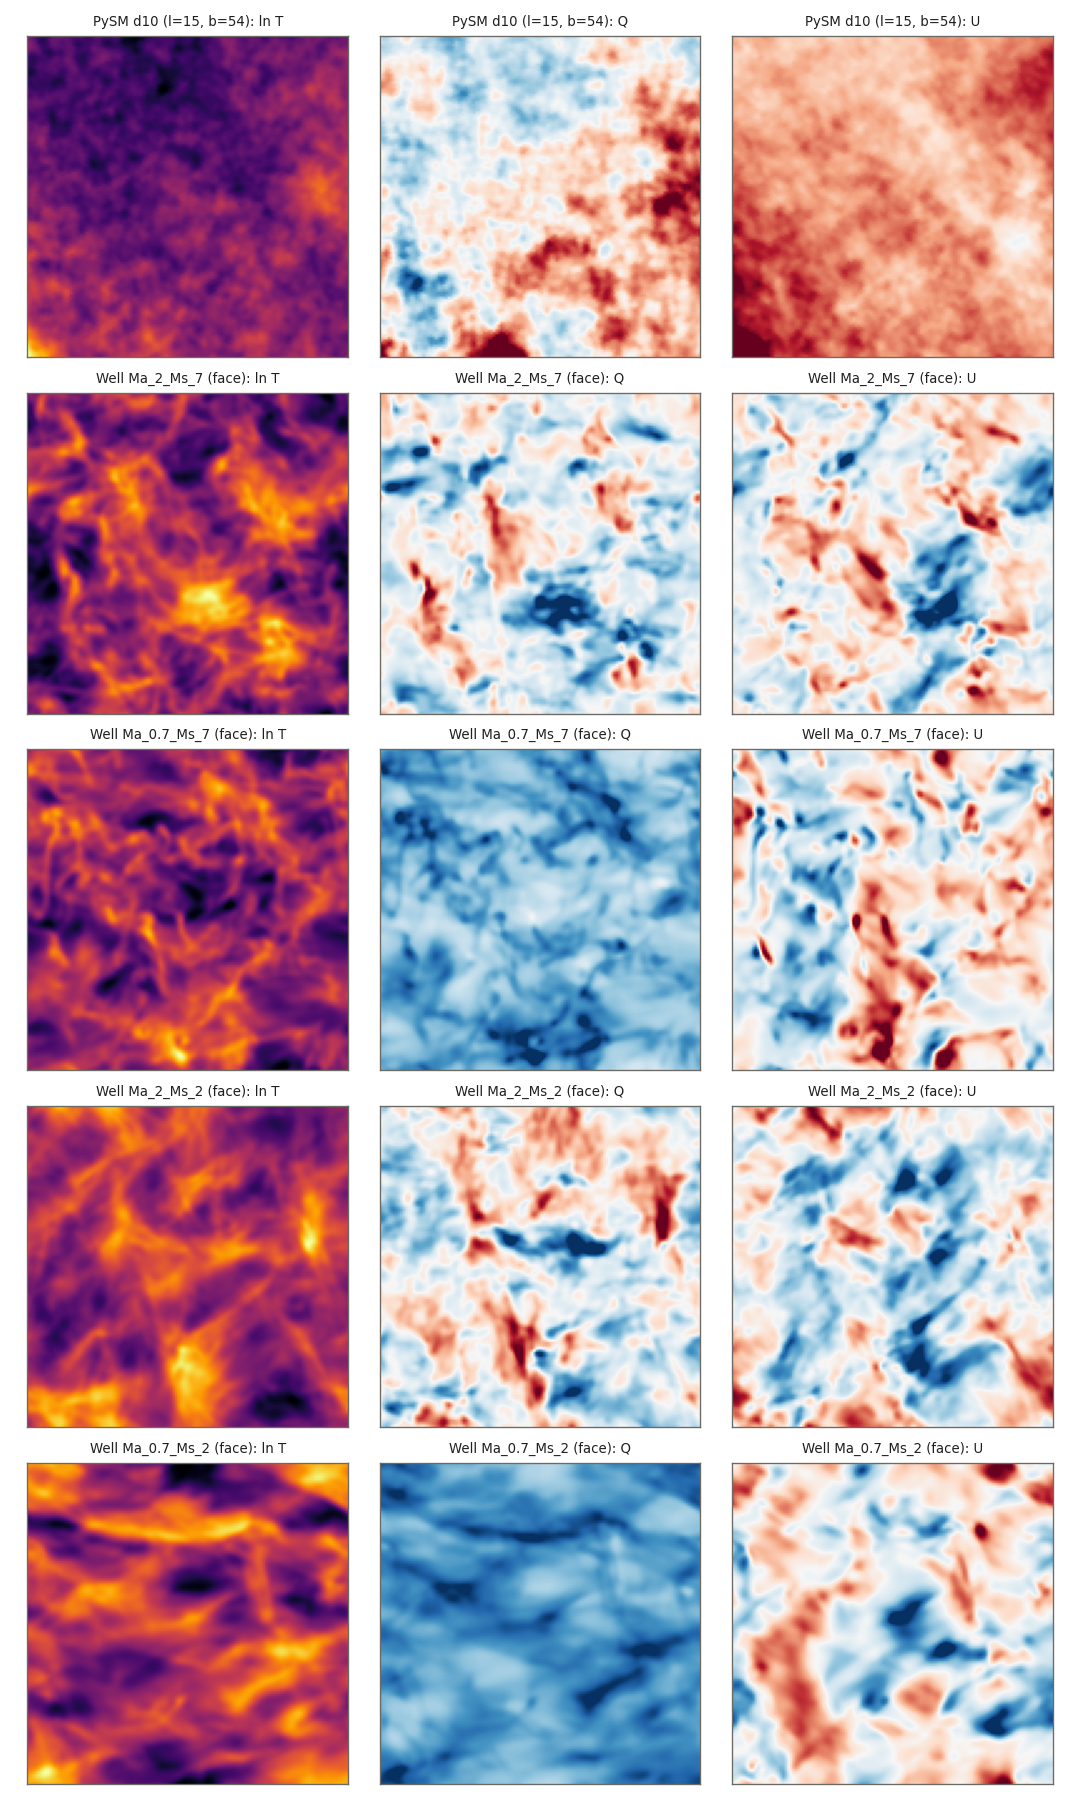
\includegraphics[width=0.60\textwidth]{../figures/well_vs_pysm/maps.png}
\caption{What the numbers describe. Top row: a PySM3 d10 patch at
$(\ell,b)=(15^\circ,54^\circ)$. Below: the four simulated faces of Section~3, same
quantities and colour scales. The simulations are visibly more filamentary, but it
is the $E$/$B$ split rather than the appearance that fails.}
\end{figure}

\end{document}
